\documentclass[9pt]{beamer}
\usetheme{boxes}
\usetheme{Boadilla}
\usecolortheme{beaver}
%\usecolortheme{sidebartab}
% \usefonttheme{structurebold}
\usefonttheme{serif}

%gets rid of bottom navigation bars
\setbeamertemplate{footline}[page number]{}

%gets rid of navigation symbols
\setbeamertemplate{navigation symbols}{}


% \usepackage{helvet}
\usepackage{amsmath, amssymb}
\usepackage{color}
%\usepackage{asymptote}
\usepackage{mathrsfs}
\usepackage{dsfont}
\usepackage{url}
\usepackage{cancel}
\usepackage{tikz}
\usetikzlibrary{fit,positioning}
\usetikzlibrary{shapes,matrix,decorations.markings,arrows}
\usetikzlibrary{graphs}
\usepackage{bbm}
\def\ind{\mathbbm{1}} %Indicator function


%
\definecolor{darkblue}{rgb}{0.0, 0.0, 0.55}
\setbeamercolor{title}{fg=darkblue}
\setbeamercolor{frametitle}{fg=darkblue}
\newcommand{\myitem}{\item[$\bullet$]}
\definecolor{darkgreen}{rgb}{0, 0.55, 0}


\newcommand{\LABEQ}[1]{\label{eq:#1}}%\mathtt{[eq:#1]}\qquad
\newcommand{\LABALG}[1]{\label{alg:#1}}%\mathtt{[lab:#1]}\qquad
\newcommand{\LABTAB}[1]{\label{tab:#1}}%{\tt [tab:$\text{$#1$}$]}}
\newcommand{\LABFIG}[1]{\label{fig:#1}}%{\tt [fig:$\text{$#1$}$]}}
\newcommand{\LABTHM}[1]{\label{thm:#1}}%{\tt [thm:#1]}}
\newcommand{\LABPRP}[1]{\label{prp:#1}}%{\tt [prp:#1]}}
\newcommand{\LABLEM}[1]{\label{lem:#1}}%{\tt [lem:#1]}}
\newcommand{\LABCOR}[1]{\label{cor:#1}}%{\tt [cor:#1]}}
\newcommand{\LABDFN}[1]{\label{dfn:#1}}%{\tt [dfn:#1]}}
\newcommand{\LABFNT}[1]{\label{fnt:#1}}%{\tt [fnt:#1]}}
\newcommand{\EQ}[1]{\eqref{eq:#1}}%$^{\text{\tt [#1]}}$} %used to be  %{(\ref{eq:#1})}
\newcommand{\ALG}[1]{~\ref{alg:#1}}
\newcommand{\TAB}[1]{~\ref{tab:#1}}%$^{\text{\tt [#1]}}$}
\newcommand{\FIG}[1]{\ref{fig:#1}} %$^{\text{\tt [#1]}}$}
\newcommand{\THM}[1]{~\ref{thm:#1}}%$^{\text{\tt [#1]}}$}
\newcommand{\COR}[1]{~\ref{cor:#1}}%$^{\text{\tt [#1]}}$}
\newcommand{\PRP}[1]{~\ref{prp:#1}}%$^{\text{\tt [#1]}}$}
\newcommand{\LEM}[1]{~\ref{lem:#1}}%$^{\text{\tt [#1]}}$}
\newcommand{\DFN}[1]{~\ref{dfn:#1}}%$^{\text{\tt [#1]}}$}
\newcommand{\FNT}[1]{~\ref{fnt:#1}}%$^{\text{\tt [#1]}}$}
\newcommand{\PAGEEQ}[1]{~\pageref{eq:#1}}
\newcommand{\PAGETAB}[1]{~\pageref{tab:#1}}
\newcommand{\PAGEFIG}[1]{~\pageref{fig:#1}}
\newcommand{\LABCHAP}[1]{\label{chap:#1}}%{\tt [chap:#1]}}
\newcommand{\LABSEC}[1]{\label{sec:#1}}%{\tt [sec:#1]}}
\newcommand{\LABSSEC}[1]{\label{ssec:#1}}%{\tt [ssec:#1]}}
\newcommand{\LABSSSEC}[1]{\label{sssec:#1}}%{\tt [sssec:#1]}}
\newcommand{\CHAP}[1]{~\ref{chap:#1}}%$^{\text{\tt [c:#1]}}$}
\newcommand{\SEC}[1]{~\ref{sec:#1}}%$^{\text{\tt [s:#1]}}$}
\newcommand{\SSEC}[1]{~\ref{ssec:#1}}%$^{\text{\tt [ss:#1]}}$}
\newcommand{\SSSEC}[1]{~\ref{sssec:#1}}%$^{\text{\tt [sss:#1]}}$}



\newcommand{\ve}[1]{\boldsymbol{#1}}
\newcommand{\set}[1]{\mathcal{#1}}


\def\X{\ve{X}}
\def\x{\ve{x}}
\def\y{\ve{y}}
\def\Y{\ve{Y}}
\def\S{\ve{S}}
\def\s{\ve{s}}
\def\n{\mathtt{n}}
\def\C{\mathcal{C}}
\def\H{\ve{H}}
\newcommand{\st}[1]{{e}_{#1}}		%state
\newcommand{\str}[2]{{e}_{#2,(#1)}}	
\newcommand{\St}[1]{{E}_{#1}}		%state
\def\seqst{\ve{\st{}}}
\def\seqSt{\ve{\St{}}}
\def\S{\ve{S}}		%Symbol sequence
\def\AQAM{\mathcal{A}}
\def\Aest{\mathcal{E}}
\def\chl{\mathtt{h}} %Channel length
\def\s{\ve{s}} %transmitted word of symbols
\def\sk{{s}_k} %transmitted word of symbols 
\def\hsk{\hat{\s}_k}
\def\t{\mathtt{s}}   %Word length (symbols)

\newcommand{\p}[1]{p_{_{#1}}} %pdf or pmf
\newcommand{\q}[1]{q_{_{#1}}} %pdf or pmf
\newcommand{\Iset}[1]{\mathtt{#1}} %Index set
\def\d{\text{d}}	%Differential (for integrals)


% Sum Product Algorithm

\newcommand{\mes}[2]{m_{#1\rightarrow#2}}
\newcommand{\logmes}[2]{l_{#1\rightarrow#2}}

\newcommand{\mc}[1]{\mathcal{#1}}
\def\sX{\mc{X}}

\newcommand\Def[1]{{\textbf{Definition:}\\\emph{#1}\\\begin{center} ------------------------ \end{center}}}
\newcommand\Prop[1]{{\textbf{\textcolor{red}{Property:}}\\\emph{#1}\\\begin{center} \textcolor{red}{------------------------} \end{center}}}

\newcommand{\noteB}[1]{\textbf{\textcolor{darkblue}{#1}}}

\newcommand{\noteR}[1]{\textbf{\textcolor{darkred}{#1}}}

\newcommand{\noteG}[1]{\textbf{\textcolor{darkgreen}{#1}}}

\newcommand{\snoteB}[1]{{\textcolor{darkblue}{#1}}}

\newcommand{\snoteR}[1]{{\textcolor{darkred}{#1}}}

\newcommand{\snoteG}[1]{{\textcolor{darkgreen}{#1}}}


\newcommand{\fs}[2]{#2}

\title[]{Inference over cycle-free discrete FGs}
\author[\textcolor{white}{Advanced Digital Communications}]{Introduction to Graphical Models and Inference for Communications\\\vspace*{3mm}{\small \textcolor{black}{UC3M}}
}
%\date[08/02/2016]{{08/02/2016}}
\institute{\textcolor{white}{}}

% \pgfdeclareimage[height=0.5cm]{ITW}{pics/Logo.png}
%  \logo{\pgfuseimage{ITW}}

\AtBeginSection[]
{
  \begin{frame}<beamer>{Index}
    \tableofcontents[currentsection,currentsubsection]
  \end{frame}
}

\begin{document}

\frame{
\titlepage
\thispagestyle{empty}
\begin{center}

\includegraphics[scale=0.05]{Figuras/uc3m-logo.pdf}
\end{center}
}

\frame{
\frametitle{Today}

\begin{itemize}
\item We want to perform inference over discrete probability distributions that are represented by cycle-free Factor Graphs (a.k.a. trees).
\item One critical result: inference over trees can be done at low cost $\mathcal{O}(n)$, where $n$ is the number of latent variables.
\end{itemize}


}

\frame{
\frametitle{Exact Inference: the discrete case}

Let $\X$ and $\Y$ be two discrete random vectors with joint pmf $\p{\X,\Y}(\x,\y)$ where $\x\in\set{X}^n$, $\y\in\set{Y}^m$. For a given observation $\Y=\y$, we are interested in drawing conclusions about $\X$. 

\vspace{0.5 cm}

Two basic kind of computations:

\begin{block}{}
Find the most probable realization of the posterior probability distribution: 
\begin{align*}
\hat{\x}&=\arg\max_{\x\in\set{X}^n} \p{\X|\y}(\x)=\arg\max_{\x\in\set{X}^n} \frac{\p{\Y|\x}(\y)\p{\X}(\x)}{\p{\Y}(\y)}=\arg\max_{\x\in\set{X}^n} \p{\Y|\x}(\y)\p{\X}(\x)
\end{align*}
\noteR{Complexity $\rightarrow$ $\mathcal{O}(|\set{X}|^n)$}.
\end{block}

}

\frame{
\frametitle{Exact Inference: the discrete case (II)}

\begin{block}{}
Compute the \emph{marginal} probability distribution for  $X_i\subset\{X_1,X_2,\ldots,X_n\}$:
\begin{align*}
\p{X_i|\y}(x_i)&=\sum_{\x_{\sim i}\in\set{X}^{n-1}} \p{\X|\y}(\x)=\sum_{x_i\in\set{X}^{n-1}}\frac{\p{\Y|\x}(\y)\p{\X}(\x)}{\p{\Y}(\y)}\\\nonumber
&=\frac{1}{\p{\Y}(\y)}\sum_{x_i\in\set{X}^{n-1}}\p{\Y|\x}(\y)\p{\X}(\x),
\end{align*}
\noteR{Complexity $\rightarrow$ $\mathcal{O}(|\set{X}|^n)$}.
\end{block}
}

\section{Motivation}

\frame{
\frametitle{Motivation}
Consider the random vector $\X=\{X_1,X_2,\ldots,X_5\}$ with p.m.f.
\begin{align*}
\p{\X}(\x)=\frac{1}{Z} t_1(x_1,x_2) t_2(x_2,x_3,x_4) t_3(x_3)t_4(x_4)t_5(x_4,x_5), \qquad \x\in\set{X}^5
\end{align*}
where $t_j:\set{X}^{d_j}\rightarrow \mathbb{R}^+$ for $j=1,\dots,5$.

\begin{figure}
\centering
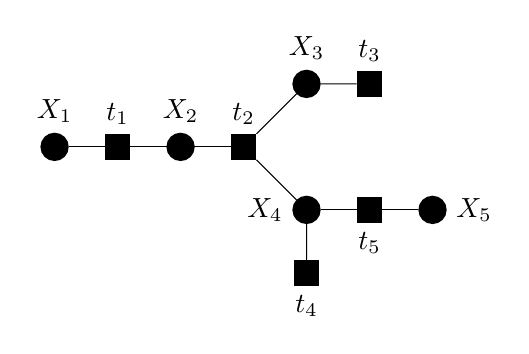
\begin{tikzpicture}[scale=0.8]
\tikzstyle{factor}=[rectangle,minimum size = 3mm, thick, draw =black,fill=black]
\tikzstyle{var}=[circle,minimum size = 3mm, thick, draw =black,fill=black]
\tikzstyle{second}=[circle, minimum size = 10mm, thick]
\tikzstyle{box}=[rectangle, draw=black!100]
\tikzstyle{connect}=[-latex, thick]
\draw[step=5cm];
	\node[var] (x_1) at (-1,0) [label=above:{$X_1$}]{};
	\node[factor] (t_1) at (0,0) [label=above:{$t_1$}]{};
	\node[var] (x_2) at (1,0) [label=above:{$X_2$}]{};
	\node[factor] (t_2) at (2,0) [label=above:{$t_2$}]{};
	\node[var] (x_3) at (3,1) [label=above:{$X_3$}]{};
	\node[factor] (t_3) at (4,1) [label=above:{$t_3$}]{};
	\node[var] (x_4) at (3,-1) [label=left:{$X_4$}]{};
	\node[factor] (t_4) at (3,-2) [label=below:{$t_4$}]{};
	\node[factor] (t_5) at (4,-1) [label=below:{$t_5$}]{};
	\node[var] (x_5) at (5,-1) [label=right:{$X_5$}]{};
	
	
	\path
		(x_1) edge []  (t_2) 
		(t_2) edge [] (x_3) 
		(x_3) edge [] (t_3)
		(t_2) edge [] (x_4)
		(t_4) edge [] (x_4)
		(x_4) edge [] (x_5);
		
\end{tikzpicture}
\end{figure}


}

\frame{

\begin{figure}
\centering
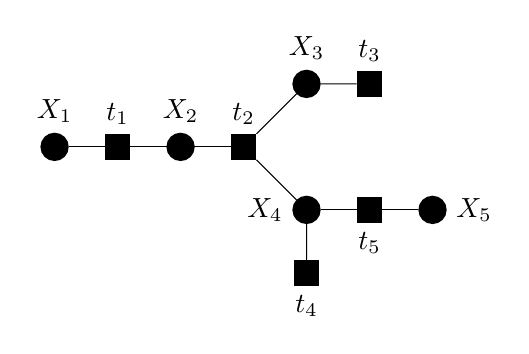
\begin{tikzpicture}[scale=0.8]
\tikzstyle{factor}=[rectangle,minimum size = 3mm, thick, draw =black,fill=black]
\tikzstyle{var}=[circle,minimum size = 3mm, thick, draw =black,fill=black]
\tikzstyle{second}=[circle, minimum size = 10mm, thick]
\tikzstyle{box}=[rectangle, draw=black!100]
\tikzstyle{connect}=[-latex, thick]
\draw[step=5cm];
	\node[var] (x_1) at (-1,0) [label=above:{$X_1$}]{};
	\node[factor] (t_1) at (0,0) [label=above:{$t_1$}]{};
	\node[var] (x_2) at (1,0) [label=above:{$X_2$}]{};
	\node[factor] (t_2) at (2,0) [label=above:{$t_2$}]{};
	\node[var] (x_3) at (3,1) [label=above:{$X_3$}]{};
	\node[factor] (t_3) at (4,1) [label=above:{$t_3$}]{};
	\node[var] (x_4) at (3,-1) [label=left:{$X_4$}]{};
	\node[factor] (t_4) at (3,-2) [label=below:{$t_4$}]{};
	\node[factor] (t_5) at (4,-1) [label=below:{$t_5$}]{};
	\node[var] (x_5) at (5,-1) [label=right:{$X_5$}]{};
	
	
	\path
		(x_1) edge []  (t_2) 
		(t_2) edge [] (x_3) 
		(x_3) edge [] (t_3)
		(t_2) edge [] (x_4)
		(t_4) edge [] (x_4)
		(x_4) edge [] (x_5);
		
\end{tikzpicture}
\end{figure}

\begin{exampleblock}{}
Assume we want to compute
\begin{align*}
\p{X_1}(x_1)=\sum_{\x\sim x_1}\p{\X}(\x)
\end{align*}
\noteR{By brute force... $|\sX|^{5}$ sums.}
\end{exampleblock}
}

\frame{
\frametitle{The variable elimination method}
\begin{block}{}
\begin{align*}
\p{X_1}(x_1)=\frac{1}{Z}\sum_{x_2,x_3,x_4,x_5\in \set{X}^4}t_1(x_1,x_2) t_2(x_2,x_3,x_4) t_3(x_3)t_4(x_4)t_5(x_4,x_5)
\end{align*}
\end{block}

\begin{itemize}
\item Distributive law ...
\end{itemize}

\begin{align*}
\p{X_1}(x_1)=\frac{1}{Z}\sum_{x_2,x_3,x_4\in \set{X}^3}t_1(x_1,x_2) t_2(x_2,x_3,x_4) t_3(x_3)t_4(x_4)\color{darkblue}\underbrace{\sum_{x_5\in\set{X}}t_5(x_4,x_5)}_{t_6(x_4)},
\end{align*}

\begin{itemize}
\item $t_6:\set{X}\rightarrow\mathbb{R}^+$ is only a function of $x_4$ and its computation for  all $x_4\in\set{X}$ requires $|\set{X}|^2$ additions.
\end{itemize}

}

\frame{
\begin{align*}\nonumber
\p{X_1}(x_1)&=\frac{1}{Z}\sum_{x_2,x_3\in \set{X}^2}t_1(x_1,x_2) t_3(x_3)\overbrace{\sum_{x_4\in\set{X}} t_2(x_2,x_3,x_4)t_4(x_4)t_6(x_4)}^{\color{darkgreen}t_7(x_2,x_3)}\\\\\nonumber
&=\frac{1}{Z}\sum_{x_2\in \set{X}}t_1(x_1,x_2) \color{darkred}\underbrace{\sum_{x_3\in\set{X}} t_3(x_3)t_7(x_2,x_3)}_{t_8(x_2)}\\\\
&=\frac{1}{Z}\color{darkblue}\underbrace{\sum_{x_2\in \set{X}}t_1(x_1,x_2) t_8(x_2)}_{t_9(x_1)}=\color{black}\frac{t_9(x_1)}{Z}
\end{align*}

\begin{block}{}
Overall, the variable elimination method computes the marginal $\p{X_1}(x_1)$ in $|\set{X}|^3+3 |\set{X}|^2$ additions.  (\noteR{Brute force $|\sX|^{5}$ sums}).
\end{block}
}

\frame{
\begin{itemize}
\item Imagine we are also interested in he marginal p.m.f. for the random variable $X_2$.
\item We could follow the same procedure and compute the marginal after $|\set{X}|^3+3 |\set{X}|^2$ additions.
\item \noteB{Good news!} Note that most of the computations needed to compute $\p{X_2}(x_2)$ coincide with those performed to compute $\p{X_1}(x_1)$!
\end{itemize}
\begin{align*}\nonumber
\p{X_2}(x_2)&=\frac{1}{Z}\sum_{x_1,x_3\in \set{X}^2}t_1(x_1,x_2) t_3(x_3)\overbrace{\sum_{x_4\in\set{X}} t_2(x_2,x_3,x_4)t_4(x_4)t_6(x_4)}^{\color{darkgreen}t_7(x_2,x_3)}\\\\\nonumber
&=\frac{1}{Z}\sum_{x_2\in \set{X}}t_1(x_1,x_2) \color{darkred}\underbrace{\sum_{x_3\in\set{X}} t_3(x_3)t_7(x_2,x_3)}_{t_8(x_2)}\\\\
&=\frac{1}{Z}\color{darkblue}\underbrace{\sum_{x_1\in \set{X}}t_1(x_1,x_2) t_8(x_2)}_{t_{10}(x_2)}=\color{black}\frac{t_{10}(x_2)}{Z}
\end{align*}


%If we additionally desire the marginal p.m.f. for the random variable $X_2$, in principle we would follow the same procedure and its computation would require $|\set{X}|^3+3 |\set{X}|^2$ additions. Nevertheless, note that most of the computations needed to compute $\p{X_2}(x_2)$ coincide with those performed in \EQ{2.4}. Indeed,
%\begin{align}\LABEQ{2.5}
%\p{X_2}(x_2)=\frac{1}{Z}\sum_{x_1\in \set{X}}t_1(x_1,x_2) t_8(x_2)
%\end{align} 
%so if we store $t_8(x_2)$ in memory when it was computed to get $\p{X_1}(x_1)$, now computing  $\p{X_2}(x_2)$ only requires $|\set{X}|^2$ additions. The rest of marginal probabilities $\p{X_i}(x_i)$ $i=3,4,5$ could be efficiently computed  by a similar procedure, reusing when possible the result of any local operation.
}

\frame{
\begin{itemize}
\item If we had store intermediate computations required to compute $\p{X_1}(x_1)$, then computing $\p{X_2}(x_2)$ \noteB{only requires $|\set{X}|^2$ additions}.
\end{itemize}
\begin{itemize}
\item What if we need to compute \noteG{all marginals $\p{X_i}(x_i)$}, $i=1,\ldots,n$?
\end{itemize}
\begin{itemize}
\item The Sum-Product algorithm (a.k.a. the BP algorithm)!
\end{itemize}

}

\section{The BP algorithm}


\frame{
\frametitle{The BP algorithm}

\begin{itemize}
\item Systematic implementation of the variable elimination procedure.
\item Efficient  computation of the the marginal probability distribution for any variable node when the joint distribution maps over a cycle-free factor graph (tree factor graph).
\end{itemize}


}


\frame{
Consider a discrete random vector $\X$ with probability distribution
\begin{align*}
\p{\X}(\x)=\frac{1}{Z}\prod_{j\in\Iset{J}}t_j(\x_{j})\qquad x_i\in\set{X},~~ i=1,\ldots,n
\end{align*}
and assume that the FG associated is a tree. 

\begin{figure}
\centering
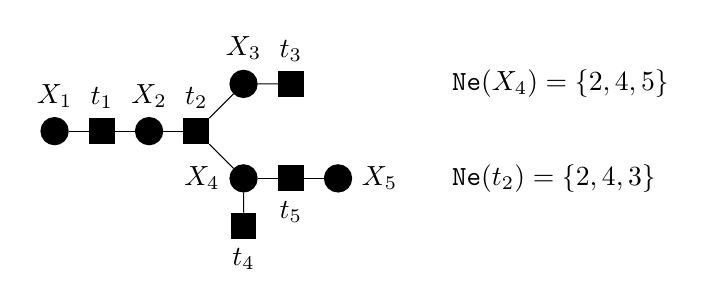
\begin{tikzpicture}[scale=0.6]
\tikzstyle{factor}=[rectangle,minimum size = 3mm, thick, draw =black,fill=black]
\tikzstyle{var}=[circle,minimum size = 3mm, thick, draw =black,fill=black]
\tikzstyle{second}=[circle, minimum size = 10mm, thick]
\tikzstyle{box}=[rectangle, draw=black!100]
\tikzstyle{connect}=[-latex, thick]
\draw[step=5cm];
	\node[var] (x_1) at (-1,0) [label=above:{$X_1$}]{};
	\node[factor] (t_1) at (0,0) [label=above:{$t_1$}]{};
	\node[var] (x_2) at (1,0) [label=above:{$X_2$}]{};
	\node[factor] (t_2) at (2,0) [label=above:{$t_2$}]{};
	\node[var] (x_3) at (3,1) [label=above:{$X_3$}]{};
	\node[factor] (t_3) at (4,1) [label=above:{$t_3$}]{};
	\node[var] (x_4) at (3,-1) [label=left:{$X_4$}]{};
	\node[factor] (t_4) at (3,-2) [label=below:{$t_4$}]{};
	\node[factor] (t_5) at (4,-1) [label=below:{$t_5$}]{};
	\node[var] (x_5) at (5,-1) [label=right:{$X_5$}]{};
	
     \node[] () at (7,1) [label=right:{$\Iset{Ne}(X_4)=\{2,4,5\}$}]{};
	\node[] () at (7,-1) [label=right:{$\Iset{Ne}(t_2)=\{2,4,3\}$}]{};

	\path
		(x_1) edge []  (t_2) 
		(t_2) edge [] (x_3) 
		(x_3) edge [] (t_3)
		(t_2) edge [] (x_4)
		(t_4) edge [] (x_4)
		(x_4) edge [] (x_5);
		
\end{tikzpicture}
\end{figure}


\begin{itemize}
\item $\Iset{Ne}(X_i)$ represents the index set of those factor nodes connected to the variable node $X_i$.
\item $\Iset{Ne}(t_j)$ the index set of those variable nodes connected to the factor node $t_j$
\end{itemize}




}

\frame{
\frametitle{A message-passing iterative algorithm}

\begin{block}{}
Local computations are regarded as \emph{messages}  between the nodes in the probabilistic graph.
\end{block}

\begin{exampleblock}{}
\noteB{$\mes{x_i}{t_j}(x_i)$} denotes the message sent from node $X_i$ to factor node $t_j$.
\end{exampleblock}

\begin{exampleblock}{}
\noteB{$\mes{t_j}{x_i}(x_i)$} denotes the message sent from factor node $t_j$ to variable node $X_i$
\end{exampleblock}

\vspace{0.5cm}

\begin{itemize}
\item Both  messages are indeed functions of $X_i$, namely each message is a stored table of $|\set{X}|$ values.
\item At each iteration, messages are updated following simple \noteB{update rules} according to a valid \noteG{schedule}.
\end{itemize}
}

\frame{
\frametitle{Update rules}
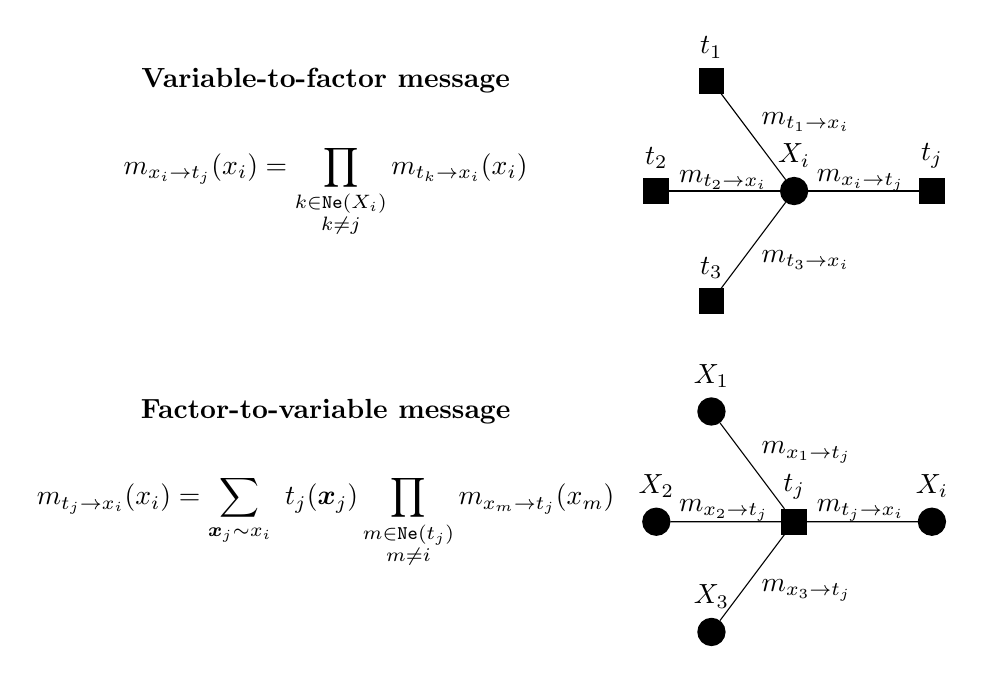
\begin{tikzpicture}[scale=0.7]
\tikzstyle{factor}=[rectangle,minimum size = 3mm, thick, draw =black, node distance = 16mm,fill=black]
\tikzstyle{var}=[circle,minimum size = 3mm, thick, draw =black, node distance = 16mm,fill=black]
\tikzstyle{second}=[circle, minimum size = 10mm, thick, node distance = 5mm]
\tikzstyle{box}=[rectangle, draw=black!100]
\tikzstyle{connect}=[-latex, thick]
\node[second] at (-6,2) [label=center:{\textbf{Variable-to-factor message}}]{};
\node[second] at (-6,0) [label=center:{$\displaystyle\mes{x_i}{t_j}(x_i)=\prod_{\substack{k\in\Iset{Ne}(X_i) \\ k\neq j}}\mes{t_k}{x_i}(x_i)$}]{};
%\node[second] at (-6,-2) [label=center:{\color{darkred}{$|\Iset{Ne}(X_i)|\times |\set{X}|$ pointwise multiplications}}]{};

\node[factor] (t_1) at (1,2) [label=above:$t_1$]{};
\node[factor] (t_2) at (0,0) [label=above:$t_2$]{};
\node[factor] (t_3) at (1,-2) [label=above:$t_3$]{};
\node[var] (x_i) at (2.5,0) [label=above:$X_i$]{};
\node[factor] (t_j) at (5,0) [label=above: $t_j$]{};
\node[second] (m1i) at (1,1.25) [label=right: $\mes{t_1}{x_i}$]{};
\node[second] (m2i) at (1,-1.25) [label=right: $\mes{t_3}{x_i}$]{};
\node[second] (m3i) at (-0.5,0.2) [label=right: $\mes{t_2}{x_i}$]{};
\node[second] (m4i) at (2,0.2) [label=right: $\mes{x_i}{t_j}$]{};

\path
	(t_1) edge (x_i)
	(t_2) edge (x_i)
	(t_3) edge (x_i)
	(x_i) edge (t_j);

\node[second] at (-6,-4) [label=center:{\textbf{Factor-to-variable message}}]{};
\node[second] at (-6,-6) [label=center:{$\displaystyle\mes{t_j}{x_i}(x_i)=\sum_{\x_{j}\sim x_i}~ t_j(\x_{j})\prod_{\substack{m\in \Iset{Ne}(t_j) \\ m\neq i}}\mes{x_m}{t_j}(x_m)$}]{};
%\node[second] at (-6,-8) [label=center:{\color{darkred}{$|\Iset{Ne}(X_i)|\times |\set{X}|$ pointwise multiplications}}]{};
%\node[second] at (-6,-8) [label=center:{\color{darkred}{$|\Iset{Ne}(X_i)|^|\set{X}|$ additions}}]{};
\node[var] (t_12) at (1,-4) [label=above:$X_1$]{};
\node[var] (t_22) at (0,-6) [label=above:$X_2$]{};
\node[var] (t_32) at (1,-8) [label=above:$X_3$]{};
\node[factor] (x_i2) at (2.5,-6) [label=above:$t_j$]{};
\node[var] (t_j2) at (5,-6) [label=above: $X_i$]{};
\node[second] (m1i) at (1,-4.75) [label=right: $\mes{x_1}{t_j}$]{};
\node[second] (m2i) at (1,-7.25) [label=right: $\mes{x_3}{t_j}$]{};
\node[second] (m3i) at (-0.5,-5.8) [label=right: $\mes{x_2}{t_j}$]{};
\node[second] (m4i) at (2,-5.8) [label=right: $\mes{t_j}{x_i}$]{};

\path
	(t_12) edge (x_i2)
	(t_22) edge (x_i2)
	(t_32) edge (x_i2)
	(x_i2) edge (t_j2);
		
\end{tikzpicture}

}

\frame{
\frametitle{Update rules}
\begin{tikzpicture}[scale=0.7]
\tikzstyle{factor}=[rectangle,minimum size = 3mm, thick, draw =black, node distance = 16mm,fill=black]
\tikzstyle{var}=[circle,minimum size = 3mm, thick, draw =black, node distance = 16mm,fill=black]
\tikzstyle{second}=[circle, minimum size = 10mm, thick, node distance = 5mm]
\tikzstyle{box}=[rectangle, draw=black!100]
\tikzstyle{connect}=[-latex, thick]
\node[second] at (-6,2) [label=center:{\textbf{Variable-to-factor message}}]{};
\node[second] at (-6,0) [label=center:{$\displaystyle\mes{x_i}{t_j}(x_i)=\prod_{\substack{k\in\Iset{Ne}(X_i) \\ k\neq j}}\mes{t_k}{x_i}(x_i)$}]{};
\node[second] at (-6,-2) [label=center:{\color{darkred}{$|\Iset{Ne}(X_i)|\times |\set{X}|$ non-trivial multiplications}}]{};

\node[factor] (t_1) at (1,2) [label=above:$t_1$]{};
\node[factor] (t_2) at (0,0) [label=above:$t_2$]{};
\node[factor] (t_3) at (1,-2) [label=above:$t_3$]{};
\node[var] (x_i) at (2.5,0) [label=above:$X_i$]{};
\node[factor] (t_j) at (5,0) [label=above: $t_j$]{};
\node[second] (m1i) at (1,1.25) [label=right: $\mes{t_1}{x_i}$]{};
\node[second] (m2i) at (1,-1.25) [label=right: $\mes{t_3}{x_i}$]{};
\node[second] (m3i) at (-0.5,0.2) [label=right: $\mes{t_2}{x_i}$]{};
\node[second] (m4i) at (2,0.2) [label=right: $\mes{x_i}{t_j}$]{};

\path
	(t_1) edge (x_i)
	(t_2) edge (x_i)
	(t_3) edge (x_i)
	(x_i) edge (t_j);

\node[second] at (-6,-4) [label=center:{\textbf{Factor-to-variable message}}]{};
\node[second] at (-6,-6) [label=center:{$\displaystyle\mes{t_j}{x_i}(x_i)=\sum_{\x_{j}\sim x_i}~ t_j(\x_{j})\prod_{\substack{m\in \Iset{Ne}(t_j) \\ m\neq i}}\mes{x_m}{t_j}(x_m)$}]{};
\node[second] at (-6,-8) [label=center:{\color{darkred}{$|\Iset{Ne}(t_j)|\times |\set{X}|$  non-trivial multiplications}}]{};
\node[second] at (-6,-9) [label=center:{\color{darkred}{$|\Iset{Ne}(t_j)|^{|\set{X}|}$ additions}}]{};
\node[var] (t_12) at (1,-4) [label=above:$X_1$]{};
\node[var] (t_22) at (0,-6) [label=above:$X_2$]{};
\node[var] (t_32) at (1,-8) [label=above:$X_3$]{};
\node[factor] (x_i2) at (2.5,-6) [label=above:$t_j$]{};
\node[var] (t_j2) at (5,-6) [label=above: $X_i$]{};
\node[second] (m1i) at (1,-4.75) [label=right: $\mes{x_1}{t_j}$]{};
\node[second] (m2i) at (1,-7.25) [label=right: $\mes{x_3}{t_j}$]{};
\node[second] (m3i) at (-0.5,-5.8) [label=right: $\mes{x_2}{t_j}$]{};
\node[second] (m4i) at (2,-5.8) [label=right: $\mes{t_j}{x_i}$]{};

\path
	(t_12) edge (x_i2)
	(t_22) edge (x_i2)
	(t_32) edge (x_i2)
	(x_i2) edge (t_j2);
		
\end{tikzpicture}

}

\frame{
\frametitle{Updating message schedule}

Messages will be updated according to a valid updating message schedule. Any updated schedule must satisfy the following:
\begin{enumerate}
\item After initialization, a message is sent for the first time from a node only when that node has received all requisite messages.
\item A message is updated and resent from a node to all its neighbours only when that node has received an updated incoming message. 
\end{enumerate}



\begin{exampleblock}{}
\noteB{Convergence is guaranteed for any tree factor graph.} After convergence, the marginal p.m.f. $\p{X_i}(x_i)$ for $i=1,\ldots,n$ can be computed as 
\begin{align*}
\p{X_i}(x_i)=\frac{1}{Z_i}\prod_{k\in\Iset{Ne}(X_i)}\mes{t_k}{x_i}(x_i),
\end{align*}
where the normalization constant is trivially obtained using the fact that the marginal must sum up to 1. 

\end{exampleblock}

}

\frame{
\frametitle{Initialization}
Two common choices

\begin{itemize}
\item \noteB{Initialization at the leaf nodes.} Leaf nodes broadcast their messages to their respective neighbors from the start. Messages are initialized as follows:
\begin{align*}
\text{For all leaf variable nodes: }~~ &\mes{x_i}{t_j}(x_i)=1\\
\text{For all leaf factor nodes: }~~ &\mes{t_j}{x_i}(x_i)=\sum_{\x_{j}\sim x_i}~ t_j(\x_{t_j})
\end{align*}

%Messages will flow through the tree, one in each direction along every edge, and after a number of steps equal to the diameter of the graph, every message will have been created.

\item \noteB{Global initialization.}  We set  all the initial messages from variables to 1.
\begin{align*}
\text{For all variable nodes: }~~ &\mes{x_i}{t_j}(x_i)=1~~ x_i\in\set{X}
\end{align*}
\end{itemize}


}

\frame{
\frametitle{Initialization}

\begin{itemize}
\item \noteB{Initialization at the leaf nodes.} \noteR{Recommended for cycle-free FGs}.
Messages will flow through the tree, one in each direction along every edge, and after a number of steps equal to the diameter of the graph, every message will have been created.

\item \noteB{Global initialization.} Note that the global initialization leads to a load of wasted computations, whose results are gradually flushed out by the correct answer computed by the first initialization method.
\noteR{This is the standard initialization when the graph is not cycle-free}. 
\end{itemize}

}

\section{Computational aspects of the BP algorithm}

\frame{
\frametitle{Message normalization}
\begin{itemize}
\item After several iterations of the SP algorithm, the numerical value of messages can become very small and numerical precision issues can occur. 
\item \noteR{Large graphs}.
\item One simple way to fix this issue is to normalize the variable-to-factor messages so they represent a valid p.m.f. (it sums up to one):
\begin{align*}
\mes{x_i}{t_j}(x_i)=\frac{\displaystyle\prod_{\substack{k\in\Iset{Ne}(X_i) \\ k\neq j}}\mes{t_k}{x_i}(x_i)}{\displaystyle \sum_{x_i\in\set{X}}~~\prod_{\substack{k\in\Iset{Ne}(X_i) \\ k\neq j}}\mes{t_k}{x_i}(x_i)}
\end{align*}
\end{itemize}

\begin{alertblock}{}
This method avoids numerical problems but it is only valid when we are interested in computing the marginal probability distribution of the variables in the graph.
\end{alertblock}

\begin{exampleblock}{}
The BP messages can be also used to efficiently compute (or approximate) the normalization constant  $Z$. In this case, we cannot normalize the BP messages.
\end{exampleblock}

}


\frame{
\frametitle{Log-messages}
Another useful computational trick involves passing the logarithms of the messages. Define:
\begin{align*}
\logmes{x_i}{t_j}(x_i)=\log\mes{x_i}{t_j}(x_i)
\end{align*}
then the variable-to-factor update rule becomes simply:
\begin{align*}
\displaystyle\logmes{x_i}{t_j}(x_i)=\sum_{\substack{k\in\Iset{Ne}(X_i) \\ k\neq j}}\logmes{t_k}{x_i}(x_i)
\end{align*}
More care is required for the update of the factor-to-variable messages:
\begin{align*}
\displaystyle\logmes{t_j}{x_i}(x_i)=\log\left(\sum_{\x_{j}\sim x_i}~ t_j(\x_{j})\color{darkred}\exp\left(\sum_{\substack{m\in \Iset{Ne}(t_j) \\ m\neq i}}\logmes{x_m}{t_j}(x_m)\right)\color{black}\right).
\end{align*}
\begin{alertblock}{}
The exponentiation of the log messages will cause potential numerical precision problems. 
\end{alertblock}
}

\frame{
\frametitle{Log-messages (II)}
By finding the largest value of the incoming log messages, we can express the factor-to-variable update rule as follows:
\begin{align*}
\logmes{}{t_j}^*=\max_{\substack{m\in \Iset{Ne}(t_j) \\ m\neq i}} \max_{x_m\in\set{X}}\logmes{x_m}{t_j}(x_m)
\end{align*}
and then
\begin{align*}
\displaystyle\logmes{t_j}{x_i}(x_i)=\logmes{}{t_j}^*+\log\left(\sum_{\x_{j}\sim x_i}~ t_j(\x_{j})\exp\left(\sum_{\substack{m\in \Iset{Ne}(t_j) \\ m\neq i}}\logmes{x_m}{t_j}(x_m)-\logmes{}{t_j}^*\right)\right),
\end{align*}
where all exponential terms will be $\leq 1$ by construction. This ensures that the dominant numerical contributions to the summation are computed accurately.
}

%\section{Project 1: the foward/backward (BCJR) algorithm is just BP}
%\frame{
%\frametitle{Soft-output channel equalization}
%
%\begin{itemize}
%\item Consider a sequence of $\t$ i.i.d. $M$-ary  complex-valued  symbols, $\sk$, obtained by the encoding of a sequence of $\log_2(M)$ information bits.  
%\item $s_k\in\AQAM$ and $|\AQAM|=M$. Assume the energy of the constellation is equal to 1 J.
%\item  ISI channel that also introduces additive white Gaussian noise (AWGN):
%\begin{align*}
%&y_k=\sum_{i=1}^{\chl+1}h_{i}s_{k-i}+w_k\\
%&h_i:~\mathcal{R}(h_i)\sim \mathcal{N}(0,0.5), ~\mathcal{I}(h_i)\sim \mathcal{N}(0,0.5)\\
%&w_k:~\mathcal{R}(w_k)\sim \mathcal{N}(0,\sigma_w^2/2), ~\mathcal{I}(w_k)\sim \mathcal{N}(0,\sigma_w^2/2)
%\end{align*}
%\item $\text{SNR}=10\log_{10}((\chl+1)/\sigma_w^2)$.
%\item The sequence of symbols $\s$ is preceded and terminated by a sequence of $\chl$ deterministic known symbols: $s_k=s^*$ for $k\in\{\t-\chl,\ldots,-1\}$ and for $k\in\{\t+1,\ldots,\sk+\chl\}$.
%\item $\y=(y_1,y_2,\ldots,y_{\t+\chl})$ is the observation vector.
%\item $\ve{h}$ and $\sigma_w^2$ are known at the receiver (perfect CSI).
%\end{itemize}
%
%
%}
%
%\frame{
%\frametitle{Project 1}
%
%\begin{exampleblock}{}
%Given $\y$, we are interested in computing $\p{S_k|\y}(s_k)$ for $k=1,\ldots,\t$. This information will be crucial for the channel decoder.
%\end{exampleblock}
%
%
%\begin{enumerate}
%\item Implement the BP algorithm for arbitrary channel memory $\chl$,  sequence length $\t$ and QAM modulation alphabet.
%\item Use the cycle-free representation of the posterior distribution of symbosl and states $\p{\ve{E},\S}(\ve{e},\s)$.
%\item Understand why the algorithm obtained is equivalent to the forward/backward algorithm (a.k.a. BCJR in communicaitons).
%\item Evaluate the complexity in terms of $\chl$, $\t$ and $M$ and how many iterations will be needed until convergence.
%\item You can use Matlab or C code (called from Matlab using a MEX file). 
%\end{enumerate}
%
%}
%\frame{
%\frametitle{Project 1 (Cont)}
%Assume now that we have $2\times2$ MIMO channel: 2 independent users with a single antenna and 1 BTS with two antennas.
%\begin{align*}
%&y^{(1)}_k=\sum_{i=1}^{\chl+1}h^{(11)}_{i}s^{(1)}_{k-i}+h^{(21)}_{i}s^{(2)}_{k-i}+w^{(1)}_k\\
%&y^{(2)}_k=\sum_{i=1}^{\chl+1}h^{(12)}_{i}s^{(1)}_{k-i}+h^{(22)}_{i}s^{(2)}_{k-i}+w^{(2)}_k\\
%\end{align*}
%where $w^{(1)}_k$ and $w^{(2)}_k$ are independent. We observe $\y^{(1)}=(y^{(1)}_1,y^{(1)}_2,\ldots,y^{(1)}_{\t+\chl})$ and $\y^{(2)}=(y^{(2)}_1,y^{(2)}_2,\ldots,y^{(2)}_{\t+\chl})$.
% \begin{enumerate}
%\item Find a cycle-free FG representation of this scenario where the BP algorithm  provides the exact marginals $\p{S^{(i)}_k|\y^{(1)},\y^{(2)}}(s^{(i)}_k)$ for $i=1,2$ and $k=1,\ldots,\t$.
%\item Evaluate the complexity and how many iterations will be needed until convergence. 
%\item Try to generalize the discussion to a $n\times n$ MIMO channel.
%\end{enumerate}
%
%}
%
%\frame{
%\frametitle{Project 1 (Optional)}
%
%\begin{enumerate}
%\item Investigate and simulate low-complexity alternatives to exact inference in these two cases. 
%\item MMSE and ZF equalizers are described in any book on digital communications. A simple paper on this topic: \emph{Capacity analysis of frequency-selective MIMO channels with sub-optimal detectors}.
%\end{enumerate}
%
%
%
%}
\end{document}

